\newpage
\section{Слабая топология в локально выпуклом топологическом векторном пространстве. Теорема Мазура. Слабое замыкание единичной сферы в бесконечномерном линейном нормированном пространстве.}
Пусть $(X, \tau)$ --- локально выпуклое ТВП, тогда в $X^*$ мы заводим слабую* топологию $\tau_{w^*}$. Тогда $(X^*, \tau_{w^*})$ тоже локально выпуклое ТВП. Теперь мы рассматриваем $(X^*, \tau_{w^*})^*$. Про это пространство мы знаем теорему Шмульяна (\ref{th:shulian}). Так как $(X, \tau)$ --- локально выпукло, то существует $F: X \to (X^*, \tau_{w^*})^*$ --- изоморфизм. В $(X^*, \tau_{w^*})^*$ можно рассмотреть слабую* топологию, назовем ее $\tau_{w^{**}}$. Ее предбаза 
$$
\sigma_{w**} = \{V_{**}(\Phi, f , \eps) \mid \Phi \in (X^*, \tau_{w^*})^*, f \in X^*, \eps > 0\}
$$
Тогда 
\begin{definition}
	Будем называть слабой топологией в $X$ прообраз $\tau_{w^{**}}$ под действием $F$:
	$$
	\tau_w = \{F^{-1}(G)  \mid G \in \tau_{w{**}}\}
	$$
\end{definition}
По построению $\tau_w$, $F$ становится гомеморфизмом, тогда $\tau_w$ векторная локально выпуклая топология. Ее предбаза есть прообраз предбазы $\tau_{w{**}}$:
$$
V(x,f,\eps) = F^{-1}(V_{**}(F(x), f, \eps)) = \{y \in X \mid |f(x) - f(y)| < \eps \}
$$
То есть 
$$
\sigma_w = \{V(x, f, \eps) \mid x \in X, f \in X^*, \eps > 0\}
$$

\begin{theorem}[Мазур]\label{th:mazur}
	Пусть $(X,\tau)$ --- локально выпуклое ТВП и $M \subset X$ --- выпукло и $\tau$-замкнуто, тогда $M$ --- $\tau_w$-замкнуто.
\end{theorem}
\begin{proof}
	Рассмотрим $x$ из дополнения $ X \setminus M$. По теореме об отделимости \ref{th:strong_sep} точка это выпуклый компакт, $M$ выпукло и замкнуто, $M \cap \{x\} = \varnothing$ тогда они строго отделимы:
	$$
	\exists f \in X^*\setminus \{0\} \ \exists \gamma_1 < \gamma_2 \in \R\colon \forall y \in M \Rightarrow \Rea f(y) \leq \gamma_1 < \gamma_2 =\Rea f(x)
	$$
	Тогда рассмотрим окрестность $x$: $V(x,f, \gamma_2 - \gamma_1)$, покажем, что эта окрестность полностью лежит вне $M$: 
	$$
	\forall z \in V(x,f,\gamma_2 - \gamma_1) \Rightarrow |f(z) - f(x)| < \gamma_2 - \gamma_1
	$$
	Тогда 
	$$
	\Rea f(x) - \Rea f(z) \leq |f(z) - f(x)| < \gamma_2 - \gamma_1 \Rightarrow \Rea f(z) > \gamma_1 + \Rea f(x)  - \gamma_2 = \gamma_1
	$$
	Таким образом $V(x,f,\gamma_2 - \gamma_1) \subset X \setminus M$, значит $M$ --- $\tau_w$-замкнуто.
\end{proof}
\begin{next0}
	Если $(X, \|\|)$ --- ЛНП, тогда $M \subset X$ --- выпукло , то $[M]_{\|\|}$ --- слабо замкнуто, значит
	$$
	\{x_n\} \subset M\colon x_n \xrightarrow{\tau_w} y \Rightarrow  y \in [M]_{\|\|}
	$$
	Таким образом слабо сходящаяся последовательность на выпуклом множестве не может убегать далеко даже по сильной топологии.
\end{next0}
\begin{next0}
	Если $x_n \xrightarrow{\tau_w} y$, то $\exists y_m \in \conv\{x_n\}\colon y_{m} \xrightarrow{\|\|} y$
\end{next0}

\begin{next0}
	Пусть $(X, \|\|)$ --- линейное нормированное пространство. Рассмотрим $S = \{x \in X\mid \|x\|  = 1\}$, тогда $[S]_w = B_1(0)$
\end{next0}
\textbf{Историческая справка.} Станислав Мазур обладал острым юмором. Хорошо известным событием была публичная передача живого гуся молодому шведскому математику Пер Энфло в качестве награды за решение (отрицательной) проблемы существования Базиса Шаудера в каждом центральном банаховом пространстве. Подробнее см \url{https://en.wikipedia.org/wiki/Scottish_Book}

\begin{figure}[h!]
	\centering
	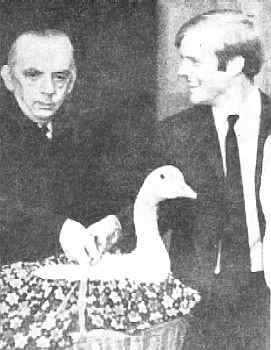
\includegraphics[scale=2]{pic/MazurGes.jpg}
\end{figure}
